

\subsection{Precision - Recall (TPR)}
\begin{figure}[H]
    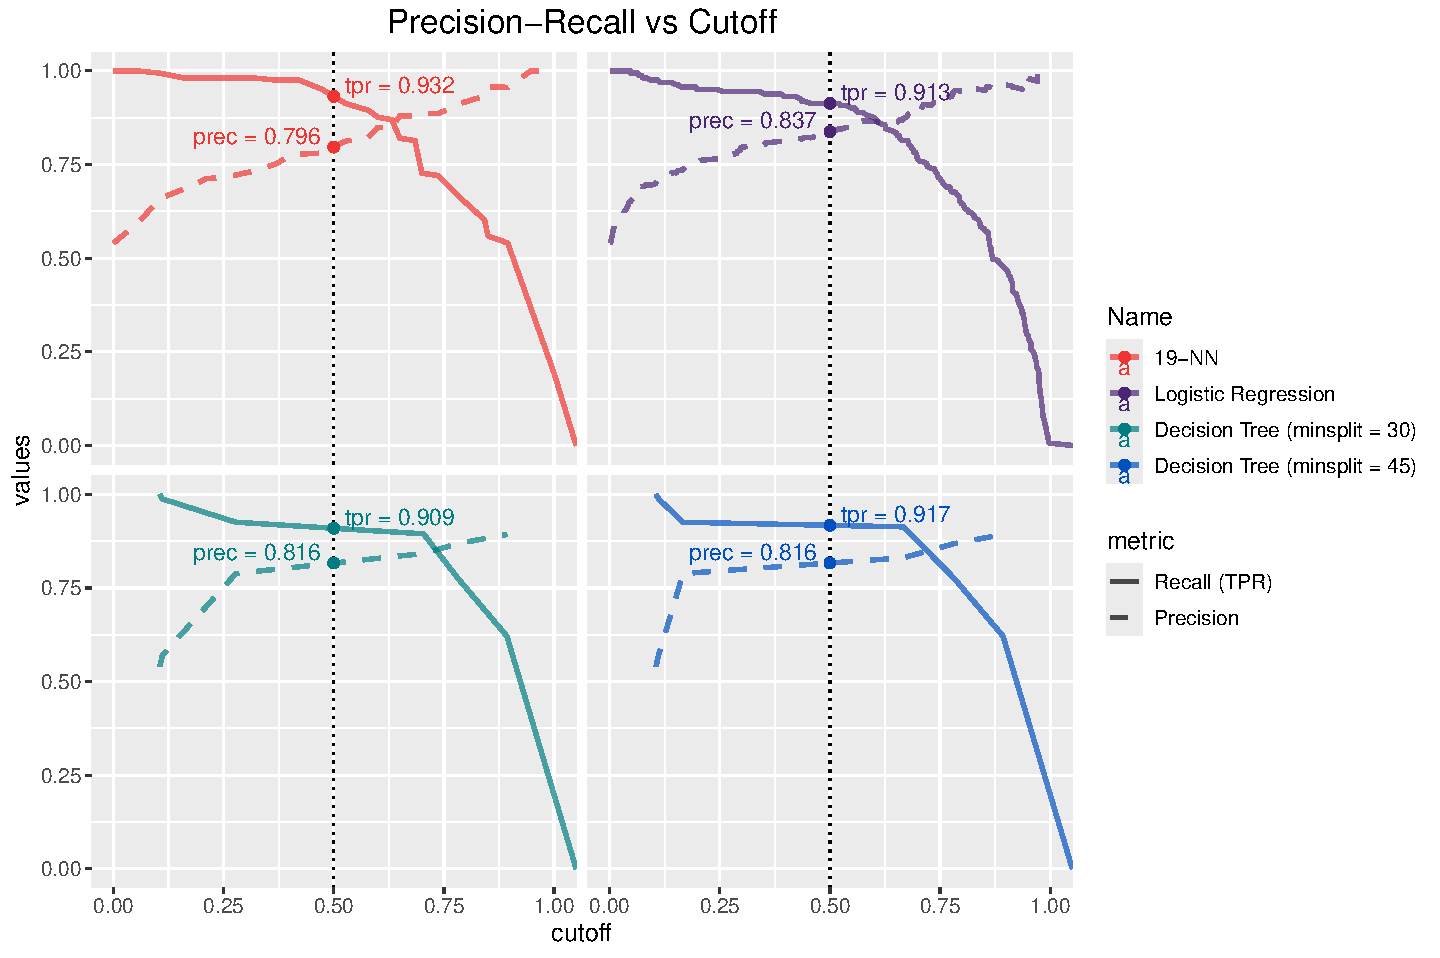
\includegraphics[width=\linewidth]{40.TPRs.pdf}
    \caption{\centering Percision/Recall -- Cutoff curves for each model}
\end{figure}

As the cutoff threshold increases, precision increases gradually whilst recall (TPR) decreases substantially, especially after the \( 0.5 \) threshold. Comparing models at the standard threshold of \( \delta = 0.5 \), it is observed that no models outperform the others in terms of precision and recall. \( 19 \)-NN tops at a \( 0.932 \) recall but fails at a low \( 0.796 \) precision, whilst logistic model observes a humble \( 0.913 \) recall but an impressive \( 0.837 \) precision. Decision trees are somewhat in between, with the \(45\)-minsplit model having a moderate \( 0.917 \) recall and \( 0.816 \) precision. 

\begin{figure}[h]
    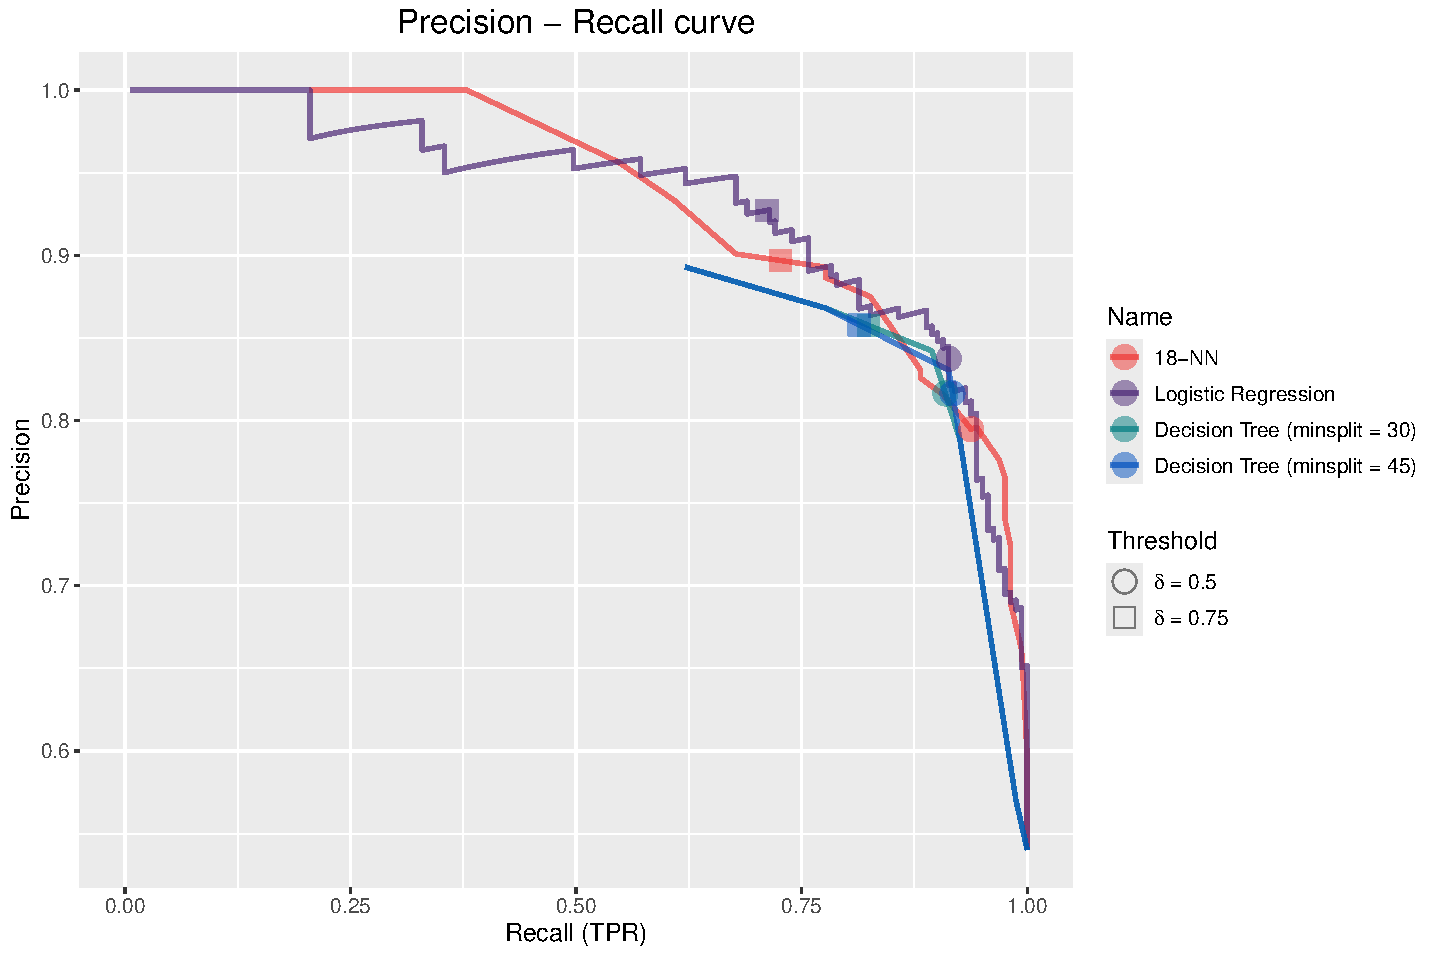
\includegraphics[width=\linewidth]{40.Precision-Recall.pdf}
    \caption{\centering Percision -- Recall curve}
\end{figure}

As the threshold is moved to \( \delta = 0.75 \), decision trees perform better in recall whilst logistic model and \( 19 \)-NN improve in precision. Concaveness around the \( \delta = 0.75 \) threshold is observed on the precision-recall curve of the \( 19 \)-NN model, whilst logistic model generally still performs well around this region.

